\setcounter{chapter}{6}
\chapter{Relative tensors, ideas of volume, Green-Stokes theorems.}
\pagebreak[4]

\section{p241 - Exercise}
\begin{tcolorbox}
If $b_{rs}$ is an absolute tensor, show that the determinant $\left|b_{rs}\right|$ is a relative invariant of weight $2$. What are the tensor characters of $\left|c^{rs}\right|$ and $\left|f^r_{s}\right|$?
\end{tcolorbox}
As $b_{rs}$ is an absolute tensor, we have 
\begin{align}
b^{'}_{uv}&= b_{rs}\pdv{x^r}{x^{'u}}\pdv{x^s}{x^{'v}}
\end{align}
Hence,
\begin{align}
\left|b^{'}_{uv}\right|&= \left|b_{rs}\right|\left|\pdv{x^r}{x^{'u}}\right|\left|\pdv{x^s}{x^{'v}}\right|
\end{align}
and as $J= \left|\pdv{x^k}{x^{'s}}\right|$ we get 
\begin{align}
\left|b^{'}_{uv}\right|&= J^2\left|b_{rs}\right|
\end{align}
Conclusion, $\left|b_{rs}\right|$ is a relative invariant of weight $ 2$.
$$\lozenge$$
As $c^{rs}$ is an absolute tensor, we have 
\begin{align}
c^{'uv}&= c^{rs}\pdv{x^{'u}}{x^r}\pdv{x^{'v}}{x^s}
\end{align}
Hence,
\begin{align}
\left|c^{'uv}\right|&= \left|c^{rs}\right|\left|\pdv{x^{'u}}{x^r}\right|\left|\pdv{x^{'v}}{x^s}\right|
\end{align}
and as $J^{-1}= \left|\pdv{x^{'s}}{x^k}\right|$ we get 
\begin{align}
\left|c^{'uv}\right|&= J^{-2}\left|c^{rs}\right|
\end{align}
Conclusion, $\left|c^{rs}\right|$ is a relative invariant of weight $ -2$.
$$\lozenge$$
As $f^{r}_{s}$ is an absolute tensor, we have 
\begin{align}
f^{'u}_{v}&= f^{r}_{s}\pdv{x^{'u}}{x^r}\pdv{x^s}{x^{'v}}
\end{align}
Hence,
\begin{align}
\left|f^{'u}_{v}\right|&= \left|f^{r}_{s}\right|\left|\pdv{x^{'u}}{x^r}\right|\left|\pdv{x^s}{x^{'v}}\right|
\end{align}
and we get 
\begin{align}
\left|f^{'u}_{v}\right|&= JJ^{-1}\left|f^{r}_{s}\right|
\end{align}
Conclusion, $\left|f^{r}_{s}\right|$ is an absolute  invariant tensor .
$$\blacklozenge$$
\newpage



\section{p242 - Exercise}
\begin{tcolorbox}
Show that, in three dimensions, the only non-vanishing components of $\delta^{kl}_{rs}$ are
$$\delta^{23}_{23}=\delta^{32}_{32}=\delta^{31}_{31}=\delta^{13}_{13}=\delta^{12}_{12}=\delta^{21}_{21}=1$$
$$\delta^{23}_{32}=\delta^{32}_{23}=\delta^{31}_{13}=\delta^{13}_{31}=\delta^{12}_{21}=\delta^{21}_{12}=-1$$
\end{tcolorbox}
This is easily seen. If $(k,l), (r, s)\ $ are considered as sets, then $\delta^{kl}_{rs}\ne 0 \quad\Leftrightarrow\quad (k,l)\ne (r, s)$.
And , $\delta^{kl}_{rs}= 1 \quad\Leftrightarrow\quad k=r \wedge l=s  $ and on the opposite $\delta^{kl}_{rs}= -1 \quad\Leftrightarrow\quad k=s \wedge l=r  $
$$\blacklozenge$$
\newpage


\section{p243 - Exercise}
\begin{tcolorbox}
Show that equations $\mathbf{5.231}$ and $\mathbf{6.128}$ can be written as follows:
$$M_{rs} = \delta^{kl}_{rs}z_kF_l$$
$$\omega_{rs} = \half\delta^{kl}_{rs}v_{l,k}$$
\end{tcolorbox}
\begin{align}
\text{(5.231)}\quad M_{rs}&=\epsilon_{rsn}M_n= z_rF_s-z_sF_r
\end{align}
In this expression $M_{rs}=0$ when $r=s$, but this is also the case with $\delta^{kl}_{rs}$.\\
In $M_{rs} = \delta^{kl}_{rs}z_kF_l$ we see that there is no contribution in the summation when $k=l$. The only contribution being those for which $k=r \wedge l=s \text{ (positive contribution) } \vee \quad k=s \wedge l=r \text{ (negative contribution) } $, hence $$\delta^{kl}_{rs}z_kF_l\quad\Leftrightarrow\quad z_rF_s-z_sF_r$$
$$\lozenge$$
\begin{align}
\text{(6.128)}\quad \omega_{rs} = \half\left(v_{s,r}-v_{r,s}\right)
\end{align}
The same arguments of the previous case apply to this case (a way to see this is to represent symbolically,  $z_rF_s$ and $v_{s,r}$ by $T_{rs}$)
$$\blacklozenge$$
\newpage


\section{p243 - Exercise}
\begin{tcolorbox}
If $T_{k_1k_2\dots k_M}$ is completely skew-symmetric, determine 
$$\delta^{k_1k_2\dots k_M}_{s_1s_2\dots s_M}T_{k_1k_2\dots k_M}$$
\end{tcolorbox}

$\delta^{k_1k_2\dots k_M}_{s_1s_2\dots s_M}T_{k_1k_2\dots k_M}$ is a sum of $M!$ terms: the first of these is $T_{s_1s_2\dots s_M}$ ; the other terms are obtained from it by permuting the subscripts and a minus sign is attached if the permutation is odd. Since $T_{s_1s_2\dots s_M}$ is completely skew-symmetric, each of the $M!$ terms equals  $+T_{s_1s_2\dots s_M}$ 
Hence,

$$ \delta^{k_1k_2\dots k_M}_{s_1s_2\dots s_M}T_{k_1k_2\dots k_M}= M! \ T_{s_1s_2\dots s_M}$$
$$\blacklozenge$$
\newpage



\section{p245 - Exercise}
\begin{tcolorbox}
Show that $\epsilon^{r_1r_2\dots r_N}\epsilon_{r_1r_2\dots r_N}= N!$ .
\end{tcolorbox}
First note that $sign(\epsilon^{r_1r_2\dots r_N})=sign(\epsilon_{r_1r_2\dots r_N})$ so that each term in the summation is always $+1$.\\
There are $N$ choices to chose from for $r_1$, $N-1$ for $r_2$ , etc. and only one for $r_N$. And so $\epsilon^{r_1r_2\dots r_N}\epsilon_{r_1r_2\dots r_N}= N!$ 
$$\blacklozenge$$
\newpage




\section{p245 - Clarification to 7.113 }
\begin{tcolorbox}
$$\epsilon^{k_1\dots k_M r_1\dots r_{N-M}}\epsilon_{s_1\dots s_M r_1\dots r_{N-M}}= \left(N-M\right)!\ \delta^{k_1\dots k_M}_{s_1\dots s_M}$$
\end{tcolorbox}
This can be seen as followed.\\
As the permutation $\left(r_1\dots r_{N-M}\right) $ is the same for both covariant and contravariant permutation symbols, the product $\epsilon^{k_1\dots k_M r_1\dots r_{N-M}}\epsilon_{s_1\dots s_M r_1\dots r_{N-M}}$ for a fixed permutation $\left(r_1\dots r_{N-M}\right) $ (i.e. no summation on repeated indexes) will be determined by $\delta^{k_1\dots k_M}_{s_1\dots s_M} $ .Indeed,  the difference in "oddness" between  $(k_1\dots k_M r_1\dots r_{N-M})$ and $(s_1\dots s_M r_1\dots r_{N-M})$  is only determined by the difference in "oddness" between  $(k_1\dots k_M r_1)$ and $(s_1\dots s_M )$. So each term in the summation has the same contribution, i.e.; $\delta^{k_1\dots k_M}_{s_1\dots s_M} $ .

There are $M$ choices to chose from for $r_1$, $M-1$ for $r_2$ , etc. and only one for $r_M$. And so $$\epsilon^{k_1\dots k_M r_1\dots r_{N-M}}\epsilon_{s_1\dots s_M r_1\dots r_{N-M}}= \left(N-M\right)!\ \delta^{k_1\dots k_M}_{s_1\dots s_M}$$
$$\blacklozenge$$
\newpage




\section{p245 - Exercice }
\begin{tcolorbox}
If $T_{rs}$  is an absolute skew-symmetric tensor in a $4-$space, show that $$T_{14}T_{23}+T_{24}T_{31}+T_{34}T_{12}$$ is a tensor density
\end{tcolorbox}
Be $P= T_{14}T_{23}+T_{24}T_{31}+T_{34}T_{12}$, we can write this as $P= \frac{1}{8}\delta^{ijmn}_{1234}T_{ij}T_{mn}$ 
\begin{figure}[H]%
    \centering
    \subfloat[]{
\begin{tikzpicture}[scale=1]
\coordinate (p1) at (2,5) {} {};
\coordinate (p2) at (3,5) {};
\coordinate (p3) at (4,5) {} {} {};
\coordinate (p4) at (5,5) {} {} {};
\coordinate (l1) at (2.5,5) {} {};
\coordinate (l2) at (4.5,5) {};
\draw  (p1) circle(0.5);
\node at (p1)  {$i$};
\draw  (p2) circle(0.5);
\node at (p2)  {$j$};
\draw  (p3) circle(0.5);
\node at (p3)  {$m$};
\draw  (p4) circle(0.5);
\node at (p4)  {$n$};
\draw  (l1) circle(1.);
\draw  (l2) circle(1.);

\draw [Latex-Latex ,dashed] plot[smooth, tension=.7] coordinates {(2,4.5) (2.5,4.3) (3,4.5)};
\draw   [Latex-Latex ,dashed]plot[smooth, tension=.7] coordinates {(4,4.5) (4.5,4.3) (5,4.5)};
\draw   [Latex-Latex ,dashed]plot[smooth, tension=.7] coordinates {(2.5,4) (3.4,3.7) (4.5,4)};
\node[anchor = south ] at (2.5,4.3)   {\tiny$P_1$};
\node[anchor = south ] at (4.5,4.3)  {\tiny$P_2$};
\node[anchor = north ] at (3.4,3.7)  {\tiny$P_3$};
\end{tikzpicture}}
\caption{Permutations}
\label{fig:fig_p247}
\end{figure}
The factor $\frac{1}{8}$ is explained by te fact that are $2^3$ possible permutations in the $i,j,m,n$ indexes i.e. $2\times2$ for the permutations $P_1$ and $P_2$ and again $2$ for the permutation $P_3$. Note that a single permutation $P_1$ or $P_2$ changes the sign of  $T_{ij}T_{mn}$ but also changes the sign of $\delta^{ijmn}_{1234}$, so the combined sign doesn't change. A double permutation $P_1$ and  $P_2$ changes the sign of  $T_{ij}$ and $T_{mn}$ resulting in a unchanged sign of  $T_{ij}T_{mn}$ but also $\delta^{ijmn}_{1234}$ is unchanged because of the double permutation. Finally $P_3$ has no effect, nor on $T_{ij}T_{mn}$ nor on $\delta^{ijmn}_{1234}$. So we have 8 repetitions for  the same set $i,j,m,n$.\\
So we have, 
\begin{align}
P&= \frac{1}{8}\delta^{ijmn}_{1234}T_{ij}T_{mn}\\
&= \frac{1}{8}\epsilon^{ijmn}T_{ij}T_{mn}
\end{align}
From this follows immediately as $\epsilon^{ijmn}$ is a relative tensor of weight $1$ and $T_{ij}$ an absolute tensor (i.e. a relative tensor of weight $0$) that $P$ is a relative tensor of eight $1$ i.e. a density.
$$\blacklozenge$$
\newpage



\section{p245 - Exercice }
\begin{tcolorbox}
Show that, for rectangular Cartesian coordinates, the vorticity tensor and the vorticity vector of a fluid are duals (cf. $\mathbf{6.130}$).
\end{tcolorbox}
$\mathbf{6.130}$:
\begin{align}
\omega_r=\half\epsilon_{rmn}\omega_{mn},\spatie \omega_{mn}=\epsilon_{rmn}\omega_r
\end{align}
Put $\hat{T}^r= \omega_r$ and $T_{mn} = \omega_{mn}$
then the expressions in $(1)$ can be expressed as (considering that the covariant an contravariant expressions are identical in rectangular Cartesian coordinates) 
\begin{align}
\hat{T}^r=\frac{1}{(3-2)!}\epsilon^{mnr}T_{mn},\spatie T_{mn}=\epsilon_{rmn}\hat{T}^r
\end{align}
which are exactly the general definitions $\mathbf{7.121}$ and $\mathbf{7.122}$ (with $N=3$ and $M=2$) for dual tensors.
$$\blacklozenge$$
\newpage



\section{p255 - Exercice }
\begin{tcolorbox}
Show that $\mathbf{7.305}$ may be written in the equivalent form
$$d\tau_{(M)}^{k_1\dots k_m}= \epsilon^{\beta_1\dots \beta_M}d_{(\beta_1)}x^{k_1}\dots d_{(\beta_M)}x^{k_M}$$
\end{tcolorbox}
The determinant of a matrix and its transpose are equal.\\
Hence we can rewrite $\mathbf{7.305} \quad \delta^{k_1\dots k_M}_{s_1\dots s_M}d_{(1)}x^{s_1}\dots d_{(M)}x^{s_M}$ as
\begin{align}
d\tau_{(M)}^{k_1\dots k_m}=\delta_{k_1\dots k_M}^{s_1\dots s_M}d_{(s_1)}x^{1}\dots d_{(s_M)}x^{M}
\end{align}
In order to be consistent with the notation we replace the $s_i$ by $\alpha_i$ as the summation occurs along the constants $c^{(i)}$
\begin{align}
d\tau_{(M)}^{k_1\dots k_m}=\delta_{k_1\dots k_M}^{\alpha_1\dots \alpha_M}d_{(\alpha_1)}x^{1}\dots d_{(\alpha_M)}x^{M}
\end{align}
Given the set $\{k_1, k_2,\dots , k_M\}$ we can represent the sequence $\{1,2,\dots , M\}$ by $\{k_j, k_m,\dots ,k_M,\dots k_n\}$ (imagine that $k_j=1, k_m=2,...$ etc.). We rewrite $(2)$ as
\begin{align}
d\tau_{(M)}^{k_1 k_2\dots k_m}=(\theta_{\alpha}) \delta_{1 2 \dots M}^{\alpha_1\dots \alpha_M}d_{(\alpha_1)}x^{k_j}d_{(\alpha_2)}x^{k_m}\dots d_{(\alpha_M)}x^{k_n}
\end{align}
where 
\begin{align}
\theta_{\alpha} = \epsilon_{k_1 k_2\dots k_M}
\end{align}
( a permutation in the lower indexes of the generalized Kronecker deltas symbol will invert the sign depending on the 'oddness' of the permutation).
Let's rearrange the product $d_{(\alpha_1)}x^{k_j}d_{(\alpha_2)}x^{k_m}\dots d_{(\alpha_M)}x^{k_n}$ so that the indexes $k_i$ are naturally ordered
\begin{align}
d\tau_{(M)}^{k_1 k_2\dots k_m}=(\theta_{\alpha}) \delta_{1 2 \dots M}^{\alpha_1\dots \alpha_M}d_{(\alpha_r)}x^{k_1}d_{(\alpha_n)}x^{k_2}\dots d_{(\alpha_1)}x^{k_n}\dots d_{(\alpha_s)}x^{k_M}
\end{align}
and changing the order in the upper indexes of the general Kroneckers delta's:
\begin{align}
d\tau_{(M)}^{k_1 k_2\dots k_m}=(\theta_{\alpha})(\theta_{k}) \delta_{1 2 \dots M}^{\alpha_r\alpha_n \dots \alpha_s}d_{(\alpha_r)}x^{k_1}d_{(\alpha_n)}x^{k_2}\dots d_{(\alpha_1)}x^{k_n}\dots d_{(\alpha_s)}x^{k_M}
\end{align}
where $\theta_{k}= \pm 1$ depending on the 'oddness' of the permutation needed to go from $\{\alpha_1\dots \alpha_M\}$ to $\{\alpha_r\alpha_n \dots \alpha_s\}$.\\
As we can see in figure $7.2$,  it's no hard to see that 
\begin{align}
\theta_{k}=\theta_{\alpha}
\end{align}
\begin{figure}[H]%
    \centering
    \subfloat[]{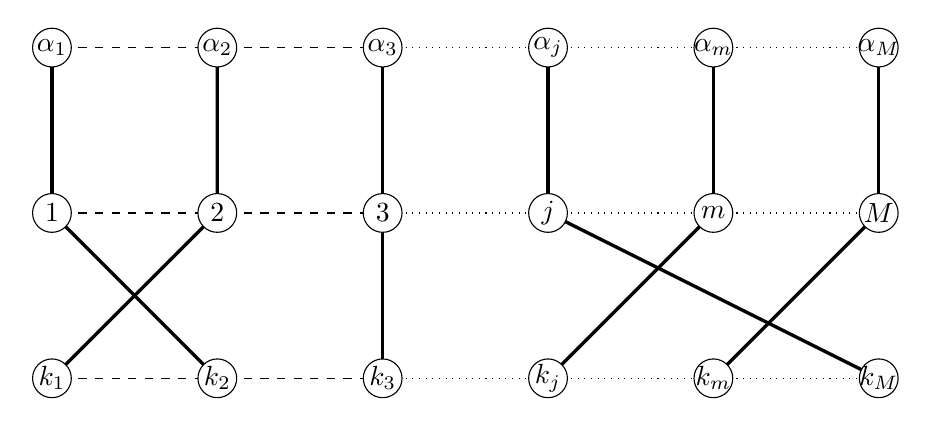
\begin{tikzpicture}[scale=0.7]


\node (alfa1) at (-10,6) {};
\node (alfaM) at (5,6) {};
\node (alfa2)at (-7,6) {};
\node (alfa3) at (-4,6) {};
\node (alfa4)at (-1,6) {};
\node (alfa5)at (2,6) {};

\node (v1) at (-10,3) {};
\node (vM) at (5,3) {};
\node (v2)at (-7,3) {};
\node (v3) at (-4,3) {};
\node (v4)at (-1,3) {};
\node (v5)at (2,3) {};

\node (k1) at (-10,0) {};
\node (kM) at (5,0) {};
\node (k2)at (-7,0) {};
\node (k3) at (-4,0) {};
\node (k4)at (-1,0) {};
\node (k5)at (2,0) {};


\draw[very thick]  (alfa1) --(v1);
\draw[very thick]  (alfa2) --(v2);
\draw[very thick]  (alfa3) --(v3);
\draw[very thick]  (alfa4) --(v4);
\draw[very thick]  (alfa5) --(v5);
\draw[very thick]  (alfaM) --(vM);
\draw[very thick]  (k2) --(v1);
\draw[very thick]  (k1) --(v2);
\draw[very thick]  (k3) --(v3);
\draw[very thick]  (kM) --(v4);
\draw[very thick]  (k4) --(v5);
\draw[very thick]  (k5) --(vM);



\draw[dashed]  (alfa1) --(alfa2);
\draw[dashed]  (alfa2) --(alfa3);
\draw[dotted]  (alfa3) --(alfa4);
\draw[dotted]  (alfa4) --(alfa5);
\draw [dotted](alfa5) --(alfaM);

\draw  [fill= white](alfa1)circle (10pt);
\draw  [fill= white](alfaM)circle (10pt);
\draw  [fill= white](alfa2)circle (10pt);
\draw  [fill= white](alfa3)circle (10pt);
\draw  [fill= white](alfa4)circle (10pt);
\draw  [fill= white](alfa5)circle (10pt);

\node[] at (alfa1)  {$\alpha_1$};
\node[] at (alfaM)  {$\alpha_M$};
\node[] at (alfa2)  {$\alpha_2$};
\node[] at (alfa3)  {$\alpha_3$};
\node[] at (alfa4)  {$\alpha_j$};
\node[] at (alfa5)  {$\alpha_m$};



\draw [dashed] (v1) --(v2);
\draw[dashed]  (v2) --(v3);
\draw[dotted]  (v3) --(v4);
\draw[dotted]  (v4) --(v5);

\draw  [dotted](v5) --(vM);
\draw  [fill= white](v1)circle (10pt);
\draw  [fill= white](vM)circle (10pt);
\draw  [fill= white](v2)circle (10pt);
\draw  [fill= white](v3)circle (10pt);
\draw  [fill= white](v4)circle (10pt);
\draw  [fill= white](v5)circle (10pt);

\node[] at (v1)  {$1$};
\node[] at (vM)  {$M$};
\node[] at (v2)  {$2$};
\node[] at (v3)  {$3$};
\node[] at (v4)  {$j$};
\node[] at (v5)  {$m$};



\draw[dashed]  (k1) --(k2);
\draw[dashed]  (k2) --(k3);
\draw[dotted]  (k3) --(k4);
\draw[dotted]  (k4) --(k5);

\draw  [dotted](k5) --(kM);
\draw  [fill= white](k1)circle (10pt);
\draw  [fill= white](kM)circle (10pt);
\draw  [fill= white](k2)circle (10pt);
\draw  [fill= white](k3)circle (10pt);
\draw  [fill= white](k4)circle (10pt);
\draw  [fill= white](k5)circle (10pt);

\node[] at (k1)  {$k_1$};
\node[] at (kM)  {$k_M$};
\node[] at (k2)  {$k_2$};
\node[] at (k3)  {$k_3$};
\node[] at (k4)  {$k_j$};
\node[] at (k5)  {$k_m$};


\end{tikzpicture}}\\
    \subfloat[]{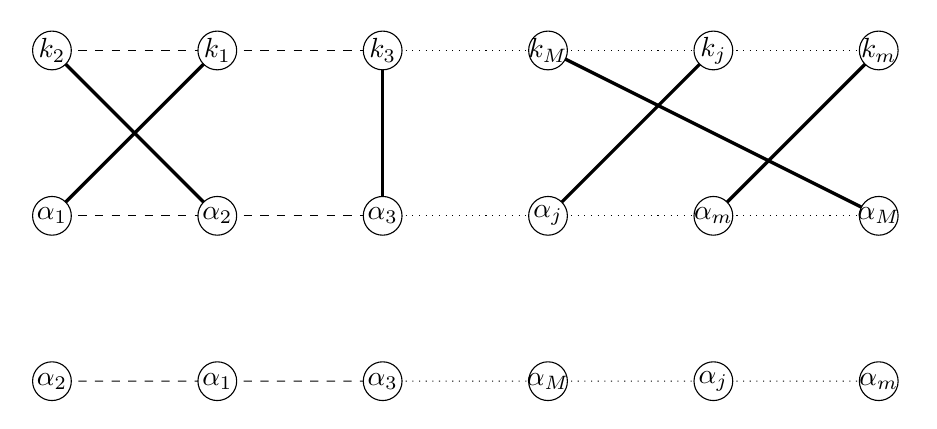
\begin{tikzpicture}[scale=0.7]


\node (alfaPR1) at (-10,-9) {};
\node (alfaPRM) at (5,-9) {};
\node (alfaPR2)at (-7,-9) {};
\node (alfaPR3) at (-4,-9) {};
\node (alfaPR4)at (-1,-9) {};
\node (alfaPR5)at (2,-9) {};

\node (alfaP1) at (-10,-6) {};
\node (alfaPM) at (5,-6) {};
\node (alfaP2)at (-7,-6) {};
\node (alfaP3) at (-4,-6) {};
\node (alfaP4)at (-1,-6) {};
\node (alfaP5)at (2,-6) {};

\node (kp1) at (-10,-3) {};
\node (kpM) at (5,-3) {};
\node (kp2)at (-7,-3) {};
\node (kp3) at (-4,-3) {};
\node (kp4)at (-1,-3) {};
\node (kp5)at (2,-3) {};



\draw[very thick]  (alfaP2) --(kp1);
\draw[very thick]  (alfaP1) --(kp2);
\draw[very thick]  (alfaP3) --(kp3);
\draw[very thick]  (alfaPM) --(kp4);
\draw[very thick]  (alfaP4) --(kp5);
\draw[very thick]  (alfaP5) --(kpM);



\draw [dashed] (kp1) --(kp2);
\draw [dashed] (kp2) --(kp3);
\draw[dotted]  (kp3) --(kp4);
\draw[dotted]  (kp4) --(kp5);
\draw  [dotted](kp5) --(kpM);

\draw  [fill= white](kp1)circle (10pt);
\draw  [fill= white](kpM)circle (10pt);
\draw  [fill= white](kp2)circle (10pt);
\draw  [fill= white](kp3)circle (10pt);
\draw  [fill= white](kp4)circle (10pt);
\draw  [fill= white](kp5)circle (10pt);

\node[] at (kp1)  {$k_2$};
\node[] at (kpM)  {$k_m$};
\node[] at (kp2)  {$k_1$};
\node[] at (kp3)  {$k_3$};
\node[] at (kp4)  {$k_M$};
\node[] at (kp5)  {$k_j$};

\draw[dashed]  (alfaP1) --(alfaP2);
\draw[dashed]  (alfaP2) --(alfaP3);
\draw[dotted]  (alfaP3) --(alfaP4);
\draw[dotted]  (alfaP4) --(alfaP5);
\draw [dotted](alfaP5) --(alfaPM);

\draw[dashed]  (alfaPR1) --(alfaPR2);
\draw[dashed]  (alfaPR2) --(alfaPR3);
\draw[dotted]  (alfaPR3) --(alfaPR4);
\draw[dotted]  (alfaPR4) --(alfaPR5);
\draw [dotted](alfaPR5) --(alfaPRM);

\draw  [fill= white](alfaP1)circle (10pt);
\draw  [fill= white](alfaPM)circle (10pt);
\draw  [fill= white](alfaP2)circle (10pt);
\draw  [fill= white](alfaP3)circle (10pt);
\draw  [fill= white](alfaP4)circle (10pt);
\draw  [fill= white](alfaP5)circle (10pt);

\draw  [fill= white](alfaPR1)circle (10pt);
\draw  [fill= white](alfaPRM)circle (10pt);
\draw  [fill= white](alfaPR2)circle (10pt);
\draw  [fill= white](alfaPR3)circle (10pt);
\draw  [fill= white](alfaPR4)circle (10pt);
\draw  [fill= white](alfaPR5)circle (10pt);

\node[] at (alfaP1)  {$\alpha_1$};
\node[] at (alfaPM)  {$\alpha_M$};
\node[] at (alfaP2)  {$\alpha_2$};
\node[] at (alfaP3)  {$\alpha_3$};
\node[] at (alfaP4)  {$\alpha_j$};
\node[] at (alfaP5)  {$\alpha_m$};

\node[] at (alfaPR1)  {$\alpha_2$};
\node[] at (alfaPRM)  {$\alpha_m$};
\node[] at (alfaPR2)  {$\alpha_1$};
\node[] at (alfaPR3)  {$\alpha_3$};
\node[] at (alfaPR4)  {$\alpha_M$};
\node[] at (alfaPR5)  {$\alpha_j$};
\end{tikzpicture}}
\caption{Permutations}
\label{fig:fig_p255}
\end{figure}
Indeed suppose, as in the example $(a)$ ,  $k_1=2, k_2=1,k_3=3, ,\dots ,k_j = m,\dots , k_m=j,\dots$ etc., so we get a sequence $\{k_2, k_1,k_3,\dots, k_m,\dots k_j,\dots\}$ as illustrated in $(b)$. But to have - with this sequence - an equivalent expression of 
$d\tau_{(M)}^{k_1 k_2\dots k_m}=(\theta_{\alpha}) \delta_{1 2 \dots M}^{\alpha_1\dots \alpha_M}d_{(\alpha_1)}x^{k_j}d_{(\alpha_2)}x^{k_m}\dots d_{(\alpha_M)}x^{k_n}$, we need to make an equivalent permutation so that $\alpha_r$ gets in the same position  as $k_r$, resulting in a new sequence $\{\alpha_2,\alpha_1,\alpha_3,\dots,\alpha_M,\dots,\alpha_j, \alpha_m\}$.\\
The number of permutations to generate $\theta_{\alpha}$ and $\theta_k$ are identical resulting in $\theta_{\alpha}\theta_k=1$.
So $(6)$ can be rewritten (noting that the $\alpha_r$ are dummy indexes and that we are free to rename them so that $r=1, n=2,\dots$) 
\begin{align}
d\tau_{(M)}^{k_1 k_2\dots k_m}= \delta_{1 2 \dots M}^{\beta_1\beta_2 \dots \beta_M}d_{(\beta_1)}x^{k_1}d_{(\beta_2)}x^{k_2}\dots d_{(\beta_n)}x^{k_n}\dots d_{(\beta_M)}x^{k_M}
\end{align}
Finally, using $\mathbf{7.114}$ 
\begin{align}
d\tau_{(M)}^{k_1 k_2\dots k_m}&= \underbrace{\epsilon_{1 2 \dots M}}_{=1}\epsilon^{\beta_1\beta_2 \dots \beta_M}d_{(\beta_1)}x^{k_1}d_{(\beta_2)}x^{k_2}\dots d_{(\beta_n)}x^{k_n}\dots d_{(\beta_M)}x^{k_M}\\
&= \epsilon^{\beta_1\beta_2 \dots \beta_M}d_{(\beta_1)}x^{k_1}d_{(\beta_2)}x^{k_2}\dots d_{(\beta_n)}x^{k_n}\dots d_{(\beta_M)}x^{k_M}
\end{align}
$$\blacklozenge$$
\newpage


\section{p257 - Exercice }
\begin{tcolorbox}
Let $x^k$ be rectangular Cartesian coordinates in Euclidean $3-$space. Introduce polar coordinates $r,\theta,\phi$ and consider the surface of the sphere $r=a$. On this sphere form the infinitesimal $2-$cell with corners $(\theta,\phi),\ (\theta+d\theta,\phi),\ (\theta,\phi+d\phi),\ (\theta+d\theta,\phi+d\phi)$. Determine the extension of this cell and interpret the rectangular components. In particular, show that the three independent components of the extension are (apart from the sign) equal to the areas obtained by normal projection of the cell onto the three rectangular planes. Does this interpretation remain valid if the sphere is replaces by some other surface?
\end{tcolorbox}
We use $\mathbf{7.312}$:
\begin{align}
d\tau_{(2)}^{k_1k_2}&= \epsilon^{\alpha_1\alpha_2}\pdv{x^{k_1}}{y^{\alpha_1}}\pdv{x^{k_2}}{y^{\alpha_2}}\left|d_{(\beta)}y^{\gamma}\right|
\end{align}
with $(y^1, y^2)= (\theta,\phi)$ giving if we take $f^{(i)}=c^{(i)} $ as $\theta=c^{(1)},\ \phi =c^{(2)} $:
\begin{align}
\left|d_{(\beta)}y^{\gamma}\right|&=\left|\begin{matrix}d_{(1)}y^{1}&d_{(1)}y^{2}\\
d_{(2)}y^{1}&d_{(2)}y^{2}\end{matrix}\right|\\
&=\left|\begin{matrix}d{\theta}&0\\
0&d{\phi}\end{matrix}\right|\\
&= d{\theta}d{\phi}
\end{align}
We also have
\begin{align}
\left\{\begin{array}{l}
x= a\sin{\theta}\cos{\phi}\\
y= a\sin{\theta}\sin{\phi}\\
z= a\cos{\theta}\\
\end{array}\right.\\
\end{align}
giving
\begin{align}
\left\{\begin{array}{l}
\pdv{x}{\theta}= a\cos{\theta}\cos{\phi}\\
\pdv{x}{\phi}= -a\sin{\theta}\sin{\phi}\\
\pdv{y}{\theta}= a\cos{\theta}\sin{\phi}\\
\pdv{y}{\phi}=  a\sin{\theta}\cos{\phi}\\
\pdv{z}{\theta}= -a\sin{\theta}\\
\pdv{z}{\phi}= 0\\
\end{array}\right.\\
\end{align}

and get 
\begin{align}
d\tau_{(2)}^{xy}&= \underbrace{\epsilon^{11}}_{=0}\pdv{x}{\theta}\pdv{y}{\theta}d{\theta}d{\phi}+\epsilon^{12}\pdv{x}{\theta}\pdv{y}{\phi}d{\theta}d{\phi}+\epsilon^{21}\pdv{x}{\phi}\pdv{y}{\theta}d{\theta}d{\phi}+\underbrace{\epsilon^{22}}_{=0}\pdv{x}{\phi}\pdv{y}{\phi}d{\theta}d{\phi}\\
&=a^2\cos{\theta}\cos{\phi}\sin{\theta}\cos{\phi}d{\theta}d{\phi}
+a^2\sin{\theta}\sin{\phi}\cos{\theta}\sin{\phi}d{\theta}d{\phi}\\
&=a^2\cos{\theta}\sin{\theta}d{\theta}d{\phi}\\
d\tau_{(2)}^{yx}&=-a^2\cos{\theta}\sin{\theta}d{\theta}d{\phi}
\end{align}
\begin{align}
d\tau_{(2)}^{xz}&= \underbrace{\epsilon^{11}}_{=0}\pdv{x}{\theta}\pdv{z}{\theta}d{\theta}d{\phi}+\epsilon^{12}\pdv{x}{\theta}\underbrace{\pdv{z}{\phi}}_{=0}d{\theta}d{\phi}+\epsilon^{21}\pdv{x}{\phi}\pdv{z}{\theta}d{\theta}d{\phi}+\underbrace{\epsilon^{22}}_{=0}\pdv{x}{\phi}\pdv{z}{\phi}d{\theta}d{\phi}\\
&=-a^2\sin^2{\theta}\sin{\phi}d{\theta}d{\phi}\\
d\tau_{(2)}^{zx}&=a^2\sin^2{\theta}\sin{\phi}d{\theta}d{\phi}
\end{align}
\begin{align}
d\tau_{(2)}^{yz}&= \underbrace{\epsilon^{11}}_{=0}\pdv{y}{\theta}\pdv{z}{\theta}d{\theta}d{\phi}+\epsilon^{12}\pdv{y}{\theta}\underbrace{\pdv{z}{\phi}}_{=0}d{\theta}d{\phi}+\epsilon^{21}\pdv{y}{\phi}\pdv{z}{\theta}d{\theta}d{\phi}+\underbrace{\epsilon^{22}}_{=0}\pdv{y}{\phi}\pdv{z}{\phi}d{\theta}d{\phi}\\
&=a^2\sin^2{\theta}\cos{\phi}d{\theta}d{\phi}\\
d\tau_{(2)}^{zy}&=-a^2\sin^2{\theta}\cos{\phi}d{\theta}d{\phi}
\end{align}
\begin{align}
d\tau_{(2)}^{xx}&= \underbrace{\epsilon^{11}}_{=0}\pdv{x}{\theta}\pdv{x}{\theta}d{\theta}d{\phi}+\epsilon^{12}\pdv{x}{\theta}\pdv{x}{\phi}d{\theta}d{\phi}+\epsilon^{21}\pdv{x}{\phi}\pdv{x}{\theta}d{\theta}d{\phi}+\underbrace{\epsilon^{22}}_{=0}\pdv{x}{\phi}\pdv{x}{\phi}d{\theta}d{\phi}\\
&=0
\end{align}

\begin{align}
d\tau_{(2)}^{yy}&= \underbrace{\epsilon^{11}}_{=0}\pdv{y}{\theta}\pdv{y}{\theta}d{\theta}d{\phi}+\epsilon^{12}\pdv{y}{\theta}\pdv{y}{\phi}d{\theta}d{\phi}+\epsilon^{21}\pdv{y}{\phi}\pdv{y}{\theta}d{\theta}d{\phi}+\underbrace{\epsilon^{22}}_{=0}\pdv{y}{\phi}\pdv{y}{\phi}d{\theta}d{\phi}\\
&=0
\end{align}

\begin{align}
d\tau_{(2)}^{zz}&= \underbrace{\epsilon^{11}}_{=0}\pdv{z}{\theta}\pdv{z}{\theta}d{\theta}d{\phi}+\epsilon^{12}\pdv{z}{\theta}\underbrace{\pdv{z}{\phi}}_{=0}d{\theta}d{\phi}+\epsilon^{21}\underbrace{\pdv{z}{\phi}}_{=0}\pdv{z}{\theta}d{\theta}d{\phi}+\underbrace{\epsilon^{22}}_{=0}\pdv{z}{\phi}\pdv{z}{\phi}d{\theta}d{\phi}\\
&=0
\end{align}
\begin{figure}[H]%
    \centering
    \subfloat[]{
%Axis Angles  
\tdplotsetmaincoords{70}{110}

%Macros  
\pgfmathsetmacro{\rvec}{7.5}  
\pgfmathsetmacro{\thetavec}{40}  
\pgfmathsetmacro{\phivec}{45}

\pgfmathsetmacro{\dphivec}{20}  
\pgfmathsetmacro{\dthetavec}{20}  

%Layers  
\pgfdeclarelayer{background} 
\pgfdeclarelayer{foreground}

\pgfsetlayers{background, main, foreground}
\begin{tikzpicture}
	[scale=0.8,
		tdplot_main_coords,
		axis/.style={->,black,thick},
		vector/.style={-stealth,black, thick},
		vector guide/.style={dashed,black,thick},
		angle/.style={black,thick}]

	%standard tikz coordinate definition using x, y, z coords
	\coordinate (O) at (0,0,0);

\tdplotsetcoord{E}{\rvec }{\thetavec}{\phivec}  
\tdplotsetcoord{F}{\rvec }{\thetavec + \dthetavec}{\phivec}  
\tdplotsetcoord{F'}{\rvec }{90}{\phivec}  \tdplotsetcoord{G}{\rvec }{\thetavec + \dthetavec}{\phivec + \dphivec}  
\tdplotsetcoord{G'}{\rvec }{90}{\phivec + \dphivec} 
\tdplotsetcoord{H}{\rvec }{\thetavec}{\phivec + \dphivec} 
    
%Axis  
\begin{pgfonlayer}{background}  
    \draw[thick,-latex] (0,0,0) -- (7,0,0) node[pos=1.1]{$x$};        
    \draw[thick,-latex] (0,0,0) -- (0,7,0) node[pos=1.05]{$y$};         
    \draw[thick,-latex] (0,0,0) -- (0,0,6) node[pos=1.05]{$z$};                   
\end{pgfonlayer}

%Help Lines  
\begin{pgfonlayer}{background}  
    %Up     
      
   
  
    %Down   
    \draw[dashed] (O) -- (F');  
    \draw[dashed] (O) -- (G');  
\end{pgfonlayer}  
\begin{pgfonlayer}{foreground}  
    %%Help Curves   
    \tdplotsetthetaplanecoords{\phivec}     
    %
    \tdplotdrawarc[dotted,tdplot_rotated_coords]{(O)}{\rvec}{\thetavec+\dthetavec}{90}{}{}
    %
    \tdplotsetthetaplanecoords{\phivec+\dphivec}    
    \tdplotdrawarc[dotted,tdplot_rotated_coords]{(O)}{\rvec}{\thetavec+\dthetavec}{90}{}{}

    %    
    \tdplotdrawarc[dotted,tdplot_main_coords]{(O)}{\rvec}{\phivec}{\phivec+\dphivec}{below, rotate=13}{} 
\end{pgfonlayer}


%Angles  
\begin{pgfonlayer}{foreground}  
    %Phi, dPhi  
    \tdplotdrawarc[-stealth]{(O)}{0.9}{0}{\phivec}{anchor=north}{$\phi$}    
    \tdplotdrawarc[-stealth]{(O)}{1.5}{\phivec}{\phivec + \dphivec}{}{} 
    \node at (1.4,1.9,0) {$\mathrm{d}\phi$};        
    \tdplotsetthetaplanecoords{\phivec}     
    %Theta, dTheta          
    \tdplotdrawarc[tdplot_rotated_coords,-stealth]{(0,0,0)}{1.2}{0}{\thetavec}{}{}      
    \node at (0,0.3,1.3) {$\theta$};    
    \tdplotdrawarc[tdplot_rotated_coords,-stealth]{(0,0,0)}{2.5}{\thetavec}{\thetavec + \dthetavec}{anchor=south west}{$\mathrm{d}\theta$}  
\end{pgfonlayer}

%Differential Volume

%%Lines  
\begin{pgfonlayer}{foreground}  
    \draw[dashed] (O) -- (E) node[midway, above left]{a};    
    \draw[dashed] (O) -- (F);    
    \draw[dashed] (O) -- (G);      
\end{pgfonlayer}   
\begin{pgfonlayer}{background}
    \draw[dashed] (O) -- (H);  
\end{pgfonlayer}

%%Curved 

 \begin{pgfonlayer}{foreground}     
    \tdplotsetthetaplanecoords{\phivec}       
    \tdplotdrawarc[tdplot_rotated_coords, thick]{(O)}{\rvec }{\thetavec}{\dthetavec + \thetavec}{}{}
    %   
    \tdplotsetthetaplanecoords{\phivec + \dphivec}  
    \tdplotdrawarc[tdplot_rotated_coords, thick]{(O)}{\rvec }{\thetavec}{\dthetavec + \thetavec}{above right}{$a\mathrm{d}\theta$}  
    %   
    \tdplotsetrotatedcoords{55}{-50.4313}{-6.4086}  
    \tdplotdrawarc[tdplot_rotated_coords, thick]{(O)}{\rvec }{0}{12.8173}{anchor=south }{$a\sin\theta\mathrm{d}\phi$}      
    %   
    \tdplotsetrotatedcoords{55}{-30.3813}{-8.6492}          
    \tdplotdrawarc[tdplot_rotated_coords, thick]{(O)}{\rvec}{0}{17.2983}{}{}  
\end{pgfonlayer}

%Fill Color 
\begin{pgfonlayer}{main}    
    %Front  
    \fill[gray, opacity=0.2] (E) to[bend left=4] (F)  to[bend left=2] (G) to[bend right=6.5] (H) to[bend right=4] cycle;   
\end{pgfonlayer}  

%\node at (E) {E};
%\node at (F) {F};
%\node at (G) {G};
%\node at (H) {H};
\end{tikzpicture}
}\\
    \subfloat[]{
%Axis Angles  
\tdplotsetmaincoords{75}{120}
%\tdplotsetmaincoords{90}{0}

%Macros  
\pgfmathsetmacro{\rvec}{7.5}  
\pgfmathsetmacro{\thetavec}{60}  
\pgfmathsetmacro{\phivec}{60}

\pgfmathsetmacro{\dphivec}{20}  
\pgfmathsetmacro{\dthetavec}{10}  

%Layers  
\pgfdeclarelayer{background} 
\pgfdeclarelayer{foreground}

\pgfsetlayers{background, main, foreground}
\begin{tikzpicture}
	[scale=1,
		tdplot_main_coords,
		axis/.style={->,black,thick},
		vector/.style={-stealth,black, thick},
		vector guide/.style={dashed,black,thick},
		angle/.style={black,thick}]

	%standard tikz coordinate definition using x, y, z coords
	\coordinate (O) at (0,0,0);

\tdplotsetcoord{E}{\rvec }{\thetavec}{\phivec}  
\tdplotsetcoord{F}{\rvec }{\thetavec + \dthetavec}{\phivec}  
\tdplotsetcoord{F'}{\rvec/3 }{90}{\phivec}  
\tdplotsetcoord{G}{\rvec }{\thetavec + \dthetavec}{\phivec + \dphivec}  
\tdplotsetcoord{G'}{\rvec /3}{90}{\phivec + \dphivec} 
\tdplotsetcoord{H}{\rvec }{\thetavec}{\phivec + \dphivec} 

%\coordinate (E") at {0,\rvec*sin(\phivec )*cos(\thetavec ),100*\rvec*cos(\phivec )};
\draw[dotted] (E) -- (Exz); 
\draw[dotted] (H) -- (Hxz) ;
\draw[dotted] (F) -- (Fxz) ;
\draw[dotted] (G) -- (Gxz) ;
\draw[thick] (Exz) -- (Hxz)-- (Gxz)-- (Fxz) -- cycle;
\draw[thick] (E) -- (H)-- (G)-- (F) -- cycle;


\draw [fill=white](E)circle (1.5pt);
    
%Axis  
\begin{pgfonlayer}{background}  
    \draw[thick,-latex] (0,0,0) -- (5,0,0) node[pos=1.1]{$x$};        
    \draw[thick,-latex] (0,0,0) -- (0,6,0) node[pos=1.05]{$y$};         
    \draw[thick,-latex] (0,0,0) -- (0,0,4.5) node[pos=1.05]{$z$};                   
\end{pgfonlayer}

%Help Lines  
\begin{pgfonlayer}{background}  
    %Up     
      
   
  
    %Down   
    \draw[dashed,ultra thin](O) -- (F');  
    \draw[dashed,ultra thin] (O) -- (G');  
\end{pgfonlayer}  

%Angles  
\begin{pgfonlayer}{foreground}  
    %Phi, dPhi  
    \tdplotdrawarc[-stealth]{(O)}{0.9}{0}{\phivec}{anchor=north}{$\phi$}    
    \tdplotdrawarc[-stealth]{(O)}{1.5}{\phivec}{\phivec + \dphivec}{}{} 
    \node at (1.4,1.9,0) {$\mathrm{d}\phi$};        
    \tdplotsetthetaplanecoords{\phivec}     
    %Theta, dTheta          
    \tdplotdrawarc[tdplot_rotated_coords,-stealth]{(0,0,0)}{1.2}{0}{\thetavec}{}{}      
    \node at (0,0.3,1.3) {$\theta$};    
    \tdplotdrawarc[tdplot_rotated_coords,-stealth]{(0,0,0)}{2.5}{\thetavec}{\thetavec + \dthetavec}{anchor=south west}{$\mathrm{d}\theta$}  
\end{pgfonlayer}

%Differential Volume

%%Lines  
\begin{pgfonlayer}{foreground}  
    \draw[dashed,ultra thin] (O) -- (E) ;%node[midway, above left]{a};    
    \draw[dashed,ultra thin](O) -- (F);    
    \draw[dashed,ultra thin](O) -- (G);      
\end{pgfonlayer}   
\begin{pgfonlayer}{background}
   \draw[dashed,ultra thin] (O) -- (H);  
\end{pgfonlayer}

%%Curved 



%Fill Color 
\begin{pgfonlayer}{main}    
    %Front  
    \fill[gray, opacity=0.2] (E) to[bend left=4] (F)  to[bend left=2] (G) to[bend right=6.5] (H) to[bend right=4] cycle;  
\fill[gray, opacity=0.2] (Exz) to[bend left=4] (Fxz)  to[bend left=2] (Gxz) to[bend right=6.5] (Hxz) to[bend right=4] cycle;      
\end{pgfonlayer}  


\node[anchor=north west] at (H) {$\quad ad\theta$};
\node[anchor=north west] at (F) {$\quad a\sin{\theta}d\phi$};
\node[anchor=south east] at (Gxz) {$ a\sin{\theta}d\theta \quad\quad \quad$};
\node[anchor=south ] at (Exz) {$a\sin{\theta}\sin{\phi}d\phi \quad\quad \quad \quad$};
\begin{pgfonlayer}{foreground}  
    %\draw[dashdotted, thick] (E) -- (Exy) ;  
    %\draw[dashdotted,thick] (E) -- (Eyz) ;  
\end{pgfonlayer} 

  

\coordinate (P) at (2.5,5.2,-0.12);
\draw [fill=white](P)circle (1.5pt);

\coordinate (P') at (2.8,6.2,-0.18);
\draw [fill=white](P')circle (1.5pt);
\draw[dashdotted,thick] (F) -- (P'); 
\draw[dashdotted,thick] (E) -- (P); 
%Angles  
\begin{pgfonlayer}{foreground}  
    %Phi, dPhi  
\tdplotsetthetaplanecoords{\thetavec} 
    \tdplotdrawarc[tdplot_rotated_coords,-stealth]{(E)}{-3.65}{1}{-24}{}{};          
\node[anchor=north east] at (P'){$\frac{\pi}{2}-\theta$};
\end{pgfonlayer}

\coordinate (Q) at (Eyz);
\draw [fill=white](Q)circle (1.5pt);

\coordinate (Q') at (0,6.7,3.73);
\draw [fill=white](Q')circle (1.5pt);
\draw[dashdotted,thick] (E) -- (Q); 
\draw[dashdotted,thick] (H) -- (Q'); 
%Angles  
\begin{pgfonlayer}{foreground}  
    %Phi, dPhi  
\tdplotsetthetaplanecoords{\thetavec} ;
    \tdplotdrawarc[-stealth]{(E)}{-3.4}{1}{-17}{}{};          
\node[anchor=south west] at (Q){$\quad\quad \frac{\pi}{2}-\phi$};
\end{pgfonlayer}
\end{tikzpicture}
}\\
    \subfloat[]{
\tdplotsetmaincoords{75}{120}
%\tdplotsetmaincoords{90}{0}

%Macros  
\pgfmathsetmacro{\rvec}{7.5}  
\pgfmathsetmacro{\thetavec}{60}  
\pgfmathsetmacro{\phivec}{60}

\pgfmathsetmacro{\dphivec}{20}  
\pgfmathsetmacro{\dthetavec}{10}  

%Layers  
\pgfdeclarelayer{background} 
\pgfdeclarelayer{foreground}

\pgfsetlayers{background, main, foreground}
\begin{tikzpicture}
	[scale=1,
		tdplot_main_coords,
		axis/.style={->,black,thick},
		vector/.style={-stealth,black, thick},
		vector guide/.style={dashed,black,thick},
		angle/.style={black,thick}]

	%standard tikz coordinate definition using x, y, z coords
	\coordinate (O) at (0,0,0);

\tdplotsetcoord{E}{\rvec }{\thetavec}{\phivec}  
\tdplotsetcoord{F}{\rvec }{\thetavec + \dthetavec}{\phivec}  
\tdplotsetcoord{F'}{\rvec/3 }{90}{\phivec}  
\tdplotsetcoord{G}{\rvec }{\thetavec + \dthetavec}{\phivec + \dphivec}  
\tdplotsetcoord{G'}{\rvec /3}{90}{\phivec + \dphivec} 
\tdplotsetcoord{H}{\rvec }{\thetavec}{\phivec + \dphivec} 

%\coordinate (E") at {0,\rvec*sin(\phivec )*cos(\thetavec ),100*\rvec*cos(\phivec )};
\draw[dotted] (E) -- (Exy); 
\draw[dotted] (H) -- (Hxy) ;
\draw[dotted] (F) -- (Fxy) ;
\draw[dotted] (G) -- (Gxy) ;
\draw[thick] (Exy) -- (Hxy)-- (Gxy)-- (Fxy) -- cycle;
\draw[thick] (E) -- (H)-- (G)-- (F) -- cycle;


\draw [fill=white](E)circle (1.5pt);
    
%Axis  
\begin{pgfonlayer}{background}  
    \draw[thick,-latex] (0,0,0) -- (5,0,0) node[pos=1.1]{$x$};        
    \draw[thick,-latex] (0,0,0) -- (0,9,0) node[pos=1.05]{$y$};         
    \draw[thick,-latex] (0,0,0) -- (0,0,4.5) node[pos=1.05]{$z$};                   
\end{pgfonlayer}

%Help Lines  
\begin{pgfonlayer}{background}  
    %Up     
      
   
  
    %Down   
    \draw[dashed,ultra thin](O) -- (F');  
    \draw[dashed,ultra thin] (O) -- (G');  
\end{pgfonlayer}  

%Angles  
\begin{pgfonlayer}{foreground}  
    %Phi, dPhi  
    \tdplotdrawarc[-stealth]{(O)}{0.9}{0}{\phivec}{anchor=north}{$\phi$}    
    \tdplotdrawarc[-stealth]{(O)}{1.5}{\phivec}{\phivec + \dphivec}{}{} 
    \node at (1.4,1.9,0) {$\mathrm{d}\phi$};        
    \tdplotsetthetaplanecoords{\phivec}     
    %Theta, dTheta          
    \tdplotdrawarc[tdplot_rotated_coords,-stealth]{(0,0,0)}{1.2}{0}{\thetavec}{}{}      
    \node at (0,0.3,1.3) {$\theta$};    
    \tdplotdrawarc[tdplot_rotated_coords,-stealth]{(0,0,0)}{2.5}{\thetavec}{\thetavec + \dthetavec}{anchor=south west}{$\mathrm{d}\theta$}  
\end{pgfonlayer}

%Differential Volume

%%Lines  
\begin{pgfonlayer}{foreground}  
    \draw[dashed,ultra thin] (O) -- (E) ;%node[midway, above left]{a};    
    \draw[dashed,ultra thin](O) -- (F);    
    \draw[dashed,ultra thin](O) -- (G);      
\end{pgfonlayer}   
\begin{pgfonlayer}{background}
   \draw[dashed,ultra thin] (O) -- (H);  
\end{pgfonlayer}

%%Curved 



%Fill Color 
\begin{pgfonlayer}{main}    
    %Front  
    \fill[gray, opacity=0.2] (E) to[bend left=4] (F)  to[bend left=2] (G) to[bend right=6.5] (H) to[bend right=4] cycle;  
\fill[gray, opacity=0.2] (Exy) to[bend left=4] (Fxy)  to[bend left=2] (Gxy) to[bend right=6.5] (Hxy) to[bend right=4] cycle;      
\end{pgfonlayer}  


\node[anchor=north west] at (H) {$\quad ad\theta$};
\node[anchor=north west] at (F) {$\quad a\sin{\theta}d\phi$};
\node[anchor=north east] at (Exy) {$ a\cos{\theta}d\theta $};
\node[anchor=north west] at (Fxy) {$ \quad \quad a\sin{\phi}d\phi $};
\begin{pgfonlayer}{foreground}  
    %\draw[dashdotted, thick] (E) -- (Exy) ;  
    %\draw[dashdotted,thick] (E) -- (Eyz) ;  
\end{pgfonlayer} 

  

\coordinate (P) at (2.5,5.2,-0.18);
\draw [fill=white](P)circle (1.5pt);

\coordinate (P') at (2.8,6.2,-0.18);
\draw [fill=white](P')circle (1.5pt);
\draw[dashdotted,thick] (F) -- (P'); 
\draw[dashdotted,thick] (E) -- (P); 
%Angles  
\begin{pgfonlayer}{foreground}  
    %Phi, dPhi  
\tdplotsetthetaplanecoords{\thetavec} 
    \tdplotdrawarc[tdplot_rotated_coords,-stealth]{(E)}{-1.25}{1}{-24}{}{};          
\node[anchor=north east] at (F){$\quad \quad \quad \frac{\pi}{2}-\theta$};
\end{pgfonlayer}


\end{tikzpicture}
}
\caption{Projections of extensions}
\label{fig:fig_p257}
\end{figure}
The quantities $d\tau_{(2)}^{xy},\ d\tau_{(2)}^{xz},  \ d\tau_{(2)}^{yz}$ are the projections of the extension on the respective Cartesian coordinates planes as can be seen in figure $7.3$ where figure $(a)$ depicts the extension (area = $a^2\sin{\theta}d\theta d\phi$) when choosing $\theta,\phi$ as the parameters $y^k$, while figure $(b)$ represents the projection of this extension on the $xz-$plane and figure $(c)$ represents the projection of this extension on the $xy-$plane.$$\lozenge$$ \\\\
\textbf{Does this interpretation remain valid if the sphere is replaces by some other surface?}
\\
The answer is no. For a two-space in Cartesian coordinates system  and with surface with parameters $(u,v)$, equation $(2)$ reduces to 
\begin{align}
d\tau_{(2)}^{xy}&= \left(\pdv{x}{u}\pdv{y}{v}-\pdv{x}{v}\pdv{y}{u}\right)dudv
\end{align}
So $d\tau_{(2)}^{xy}=0$ if $\pdv{x}{u}\pdv{y}{v}-\pdv{x}{v}\pdv{y}{u}=0$.
Consider the disk defined by the following parametric function
$$S: \left\{\mathbb{R}^2\rightarrow \mathbb{R}^3, \ S(u,v)= \left(\frac{u}{\sqrt{u^2+v^2+C}},\ \frac{v}{\sqrt{u^2+v^2+C}}, \ 1\right)\right\}$$ 
(the constant $C$ is there just to avoid the undefinedness of the surface for $(u,v) = (0,0)$). \\
It is easy to see that $\pdv{x}{u}\pdv{y}{v}-\pdv{x}{v}\pdv{y}{u}=0$, yet the surface is parallel with the $xy-$plane, which implies that the projection on the $xy-$plane of an elementary cell on $S$ will not have a zero area as can be seen in the figure hereunder. 

\begin{figure}[H]%
    \centering
    \pgfplotsset{every axis/.append style={
view={120}{20},
%axis equal image,
    %clip=false,
    %xlabel=$x$, ylabel=$y$, zlabel=$z$,
    %axis lines=middle,
    colormap={whitered}{
        color(0cm)=(white);
        color(1cm)=(black!75!gray)
    }
    %y dir=reverse,
%    axis on top
            }}
            


            
\begin{tikzpicture}[angle/.style={black,thick}]
\tikzmath{\a=0.05/sqrt(0.05*0.05+0.1*0.1);\k=1;\f=1;\u1=0;\v1=0;\u2=0;\v2=0;\u3=0;\v3=0;\u4=0;\v4=0;};
\a, \k,\u1,\v1,\u2,\v2,\u3,\v3,\u4,\v4,\f;
    %\pgfplotsset{ticks=none};
    \pgfplotsset{compat=1.12};
    \tikzset{>=latex} % for LaTeX arrow head
\begin{axis}
		[
		hide axis,clip=false,
		zmin=\k*0.5,
		zmax=\k,
			xmin=-\k,
		xmax=\k,
			ymin=-\k,
		ymax=\k,
		]
				%relevant points
	\coordinate (O) at ({ 0},{0},{0});%origin
	\coordinate (X) at ({ 2},{0},{0});%origin
	\coordinate (Y) at ({ 0},{1.5},{0});%origin
	\coordinate (Z) at ({ 0},{0},{0.4});%origin
	\draw[-Latex](O)--(X);
	\draw[-Latex](O)--(Y);
	\draw[-Latex](O)--(Z);
	\node[{anchor=south east}] at (X){$x$};
	\node[{anchor=south west}] at (Y){$y$};
	\node[{anchor=south west}] at (Z){$z$};
	\addplot3[surf,fill=gray!50,domain=-15:15,domain y=-15:15,samples=30,faceted color=black,mark=none, opacity=0.21,fill opacity = 0.5,thin]({x/sqrt(x*x*1+y*y+\f)},{y*\f/sqrt(x*x*1+y*y+\f)},{0.21});

			
 	\coordinate (Q) at ({ 0},{0},{0.21});%origin
\draw[fill=white](Q) circle(1pt)node[{anchor=north west}]{$$};; 	


	\tikzmath{\u1=0.5/sqrt(0.5*0.5+0.5*0.5+\f); \v1=0.5/sqrt(0.5*0.5+0.5*0.5+\f); 	};
	\coordinate (P0) at ({\u1},{\v1},{0.21});%origin
	\tikzmath{\u2=-0.5/sqrt(0.5*0.5+0.5*0.5+\f); \v2=0.5/sqrt(0.5*0.5+0.5*0.5+\f); 	};
	\coordinate (P1)at ({\u2},{\v2},{0.21});%origin
	\tikzmath{\u3=-0.5/sqrt(0.5*0.5+1.4*1.4+\f); \v3=1.4/sqrt(0.5*0.5+1.4*1.4+\f); 	};
	\coordinate (P2)at ({\u3},{\v3},{0.21});%origin
	\tikzmath{\u4=0.5/sqrt(0.5*0.5+1.4*1.4+\f); \v4=1.4/sqrt(0.5*0.5+1.4*1.4+\f); 	};
	\coordinate (P3)at ({\u4},{\v4},{0.21});%origin
	
		\coordinate (P0xy) at ({\u1},{\v1},{0});%origin
	\tikzmath{\u2=-0.5/sqrt(0.5*0.5+0.5*0.5+\f); \v2=0.5/sqrt(0.5*0.5+0.5*0.5+\f); 	};
	\coordinate (P1xy)at ({\u2},{\v2},{0});%origin
	\tikzmath{\u3=-0.5/sqrt(0.5*0.5+1.4*1.4+\f); \v3=1.4/sqrt(0.5*0.5+1.4*1.4+\f); 	};
	\coordinate (P2xy)at ({\u3},{\v3},{0});%origin
	\tikzmath{\u4=0.5/sqrt(0.5*0.5+1.4*1.4+\f); \v4=1.4/sqrt(0.5*0.5+1.4*1.4+\f); 	};
	\coordinate (P3xy)at ({\u4},{\v4},{0});%origin

	\draw[](P0)--(P1);
	\draw[](P1)--(P2);
	\draw[](P2)--(P3);
	\draw[](P3)--(P0);
	
	\draw[dashed](P0xy)--(P1xy);
	\draw[dashed](P1xy)--(P2xy);
	\draw[dashed](P2xy)--(P3xy);
	\draw[dashed](P3xy)--(P0xy);
	
		\draw[dotted](P0xy)--(P0);
	\draw[dotted](P1xy)--(P1);
	\draw[dotted](P2xy)--(P2);
	\draw[dotted](P3xy)--(P3);
	\draw[fill=white](P0) circle(1pt)node[{anchor=north west}]{$$};;
	\draw[fill=white](P1) circle(1pt)node[{anchor=north west}]{$$};;
	\draw[fill=white](P2) circle(1pt)node[{anchor=north west}]{$$};;
	\draw[fill=white](P3) circle(1pt)node[{anchor=north west}]{$$};;
	\draw[fill=white](P0xy) circle(1pt)node[{anchor=north west}]{$$};;
	\draw[fill=white](P1xy) circle(1pt)node[{anchor=north west}]{$$};;
	\draw[fill=white](P2xy) circle(1pt)node[{anchor=north west}]{$$};;
	\draw[fill=white](P3xy) circle(1pt)node[{anchor=north west}]{$$};;
	


		
\end{axis}
\end{tikzpicture}
\caption{A disk defined as $S: \left\{\mathbb{R}^2\rightarrow \mathbb{R}^3, \ S(u,v)= \left(\frac{u}{\sqrt{u^2+v^2+C}},\ \frac{v}{\sqrt{u^2+v^2+C}}, \ 1\right)\right\}$}
\label{fig:fig_p257}
\end{figure}
\textbf{Conclusion:} The interpretation of  $d\tau_{(2)}^{k_1k_2}$ as the projection of a cell on a axis-plane, does not hold for every surface.
$$\blacklozenge$$
\newpage




\section{p263 - Exercise}
\begin{tcolorbox}
Using polar coordinates in Euclidean $3-$space find the volume of an infinitesimal cell whose edges are tangent to the coordinate curves. Obtain the volume of a sphere by integration.
\end{tcolorbox}
For polar spherical coordinates we have
\begin{align}
\left(a_{mn}\right)&= \left(\begin{array}{lll}
1&0&0\\
0&r^2&0\\
0&0&r^2\sin^2\theta
\end{array}\right)
\end{align}
giving
\begin{align}
\left|a_{mn}\right| &= r^4\sin^2\theta
\end{align}

and using as parameters the $x^k \equiv(r,\theta,\phi)$ as parameters for the parametric surface

we get 
\begin{align}
\left|d_{(s)}x^k\right| &= \left|\begin{array}{lll}
dr&0&0\\
0&d\theta&0\\
0&0&d\phi\\
\end{array}\right|\\
&= drd\theta d\phi
\end{align}

Using $\mathbf{7.405}$:
\begin{align}
dv_{(N)}^2&= \epsilon (a)\left|a_{mn}\right|\left|d_{(s)}x^k\right|^2\\
&= r^4\sin^2\theta\left( drd\theta d\phi\right)^2
\end{align}
getting for the volume of a sphere with radius $R$:
\begin{align}
V&=8 \int_{0}^{R}\int_{0}^{\frac{\pi}{2}}\int_{0}^{\frac{\pi}{2}}dv_{(N)}\\
&= 8 \int_{0}^{R}\int_{0}^{\frac{\pi}{2}}\int_{0}^{\frac{\pi}{2}}r^2\sin\theta dr d\theta d\phi\\
&= \frac{4}{3}\pi R^3
\end{align}
$$\blacklozenge$$
\newpage




\section{p265 - Exercise}
\begin{tcolorbox}
In the relativistic theory of finite, expanding universe, the following line element is adopted:
$$ds^2=R^2\left[dr^2+\sin^2 r\left(d\theta^2+\sin^2\theta d\phi^2\right)\right]-dt^2$$
where $R=R(t)$ is a function of the "time" $t$. the ranges of the coordinates may be taken to be $0\leq r\leq \pi, \ 0 \leq \theta \leq \pi,\ 0 \leq \phi< 2\pi,\ -\infty < t < + \infty$.\\
Find the total volume of "space", i.e., of the surface $t=$ constant, and show that it varies with the "time" $t$ as $R^3(t)$.
\end{tcolorbox}
For the considered metric, we have
\begin{align}
\left(a_{mn}\right)&= \left(\begin{array}{llll}
R^2&0&0&0\\
0&R^2\sin^2r&0&0\\
0&0&R^2\sin^2 r\sin^2\theta&0\\
0&0&0&-1
\end{array}\right)
\end{align}

Using as parameters the $x^k \equiv(r,\theta,\phi)$ as parameters for the parametric surface and using $\mathbf{7.409}:\quad b_{\alpha\beta}= a_{ks}\pdv{x^k}{y^{\alpha}}\pdv{x^s}{y^{\beta}} $, we get for the $3-$space $t=$ constant
\begin{align}
\left(b_{mn}\right)&= \left(\begin{array}{lll}
R^2&0&0\\
0&R^2\sin^2r&0\\
0&0&R^2\sin^2 r\sin^2\theta
\end{array}\right)
\end{align}
giving 
\begin{align}
\left|b_{mn}\right| &= R^6\sin^4 r\sin^2\theta
\end{align}
Using $\mathbf{7.413}$:
\begin{align}
dv_{(M)}^2&= \frac{\epsilon (b)}{M!}a_{k_1s_1}\dots a_{k_M s_M}d\tau_{(M)}^{k_1\dots k_M}d\tau_{(M)}^{s_1\dots s_M}\\
&= -\frac{1}{6}a_{k_1s_1}\dots a_{k_M s_M}d\tau_{(M)}^{k_1\dots k_M}d\tau_{(M)}^{s_1\dots s_M}\\
&= -\frac{6}{6}a_{11}a_{22}a_{33}\left(\underbrace{d\tau_{(M)}^{123}}_{=dr d\theta d\phi} \right)^2\\
&= -R^6\sin^4 r\sin^2\theta\left(dr d\theta d\phi \right)^2\\
\Rightarrow \quad dv_{(M)}&=R^3\sin^2 r\sin\theta dr d\theta d\phi
\end{align}


getting for the volume of "space"  with "radius" $R$:
\begin{align}
V&= \int_{0}^{\pi}\int_{0}^{\pi}\int_{0}^{2\pi}R^3\sin^2 r\sin\theta dr d\theta d\phi\\
&= 2 R^3\pi  \int_{0}^{R}\sin^2 r dr \underbrace{\int_{0}^{\pi}\sin\theta d\theta}_{=\left. -cos\theta\right|_0^{\pi}}\\
&= 4 R^3\pi  \underbrace{\int_{0}^{R}\sin^2 r dr}_{=\left.\half\left(\theta-\half\sin (2 r)\right)\right|_0^{\pi}}\\
&=2\pi^2 R^3  
\end{align}
(the integral in $(11)$ can be found by substituting $\sin^2 r = 1-\cos^2 r$ and  using the cosine sum of angles rule $\cos\left(\alpha+\beta\right) = \cos\alpha\cos\beta-\sin\alpha\sin\beta$ with $\alpha = \beta=r$).
$$\lozenge$$
\begin{figure}[H]%
    \centering
    \subfloat[]{
            


            
<<<<<<< HEAD
\begin{tikzpicture}[scale = 0.7,angle/.style={black,thick}]
=======
\begin{tikzpicture}[scale = 0.8,angle/.style={black,thick}]
>>>>>>> adfdd13a74863c750c19cd7f30af5a98907dce92

\pgfplotsset{every axis/.append style={
view={120}{20},
%axis equal image,
    %clip=false,
    %xlabel=$x$, ylabel=$y$, zlabel=$z$,
    %axis lines=middle,
    colormap={whitered}{
        color(0cm)=(white);
        color(1cm)=(black!75!gray)
    }
    %y dir=reverse,
%    axis on top
            }}

\tikzmath{\p=360;\a=1/sqrt(0.05*0.05+0.1*0.1);\k=3;\f=1;\u1=0;\v1=0;\u2=0;\v2=0;\u3=0;\v3=0;\u4=0;\v4=0;};
\p, \a, \k,\u1,\v1,\u2,\v2,\u3,\v3,\u4,\v4,\f;
    %\pgfplotsset{ticks=none};
    \pgfplotsset{compat=1.12};
    \tikzset{>=latex} % for LaTeX arrow head
\begin{axis}
		[
		axis equal image,
		hide axis,clip=false,
		zmin=-\k,
		zmax=\k,
			xmin=-\k,
		xmax=\k,
			ymin=-\k,
		ymax=\k,
		]
				%relevant points
	\coordinate (O) at ({ 0},{0},{0});%origin
	\coordinate (X) at ({4* \k},{0},{0});%origin
	\coordinate (Y) at ({ 0},{4*\k},{0});%origin
	\coordinate (Z) at ({ 0},{0},{4*\k});%origin
	\draw[-Latex](O)--(X);
	\draw[-Latex](O)--(Y);
	\draw[-Latex](O)--(Z);

	\addplot3[surf,fill=white!50,domain=0:\p,domain y=0:\p,samples=30,faceted color=gray!50,mark=none, opacity=0.21,fill opacity = 0.45,thin]({\a*sin(x)*cos(y)},{\a*sin(x)*sin(y)},{\a*cos(x)});
	\node[{anchor=south east}] at (X){$z$};
	\node[{anchor=south west}] at (Y){$x$};
	\node[{anchor=south west}] at (Z){$w$};
			
 \coordinate (Q) at ({ 0},{0},{0.0});%origin
\draw[fill=white](Q) circle(1pt)node[{anchor=north west}]{$$};; 	
 \coordinate (Qx) at ({\a*sin(0)*cos(0)},{\a*sin(0)*sin(0)},{\a*cos(0)});%origin
 \node[{anchor=south west}] at (Qx){$r=0, \theta =\pi$};
\draw[fill=white](Qx) circle(1pt)node[{anchor=north west}]{$$};; 
 \coordinate (Qz) at ({\a*sin(90)*cos(0)},{\a*sin(90)*sin(0)},{\a*cos(90)});%origin
 \node[{anchor=south west}] at (Qz){$r=\frac{\pi}{2}, \theta =0$};
\draw[fill=white](Qz) circle(1pt)node[{anchor=north west}]{$$};; 
 \coordinate (Qw) at ({\a*sin(90)*cos(90)},{\a*sin(90)*sin(90)},{\a*cos(90)});%origin
 \node[{anchor=south west}] at (Qw){$r=\frac{\pi}{2}, \theta =\frac{\pi}{2}$};
\draw[fill=white](Qw) circle(1pt)node[{anchor=north west}]{$$};; 


\draw[dashed] plot[variable=\x,domain=0:\p/4,samples=30,thick]({\a*sin(\x)*cos(0)},{\a*sin(\x)*sin(0)},{\a*cos(\x)});

\draw [postaction=decorate,decoration={markings,
    mark=at position 1 with {\arrow{Latex}}}] plot[variable=\x,domain=0:\p/9,samples=30,thick]({\a*sin(\x)*cos(60)},{\a*sin(\x)*sin(60)},{\a*cos(\x)});
 \coordinate (Pp) at ({\a*sin(\p/9)*cos(60)},{\a*sin(\p/9)*sin(60)},{\a*cos(\p/9)});
\draw[fill=white](Pp) circle(1.5pt)node[{anchor=west}]{$\phi =0$};; 

\draw [postaction=decorate,decoration={markings,
    mark=at position 1 with {\arrow{Latex}}}] plot[variable=\x,domain=0:\p/9,samples=30,thick]({\a*sin(\x)*cos(60)},{-\a*sin(\x)*sin(60)},{\a*cos(\x)});

\coordinate (Pn) at ({\a*sin(\p/9)*cos(60)},{-\a*sin(\p/9)*sin(60)},{\a*cos(\p/9)});
\draw[fill=white](Pn) circle(1.5pt)node[{anchor=east}]{$\phi =\pi$};; 

\draw[postaction=decorate,decoration={markings,
    mark=at position 1 with {\arrow{Latex}}}] plot[variable=\x,domain=0:60,samples=30,thick]({\a*sin(\p/9)*cos(\x)},{\a*sin(\p/9)*sin(\x)},{\a*cos(\p/9)});
\draw [postaction=decorate,decoration={markings,
    mark=at position 1 with {\arrow{Latex}}}] plot[variable=\x,domain=0:60,samples=30,thick]({\a*sin(\p/9)*cos(\x)},{-\a*sin(\p/9)*sin(\x)},{\a*cos(\p/9)});
 \coordinate (Pm) at ({\a*sin(\p/9)*cos(0)},{-\a*sin(\p/9)*sin(0)},{\a*cos(\p/9)});
\draw[fill=white](Pm) circle(1.5pt)node[{anchor= west}]{$$};; 

 \coordinate (Ta) at ({\a*sin(\p/9)*cos(30)},{\a*sin(\p/9)*sin(30)},{\a*cos(\p/9)});%origin
\draw[white,fill=white](Ta) circle(10pt)node[black]{$\theta$};; 

\coordinate (Tb) at ({\a*sin(\p/9)*cos(30)},{-\a*sin(\p/9)*sin(30)},{\a*cos(\p/9)});%origin
\draw[white,fill=white](Tb) circle(10pt)node[black]{$\theta$};; 

 \coordinate (Tc)  at ({\a*sin(\p/9/2)*cos(60)},{\a*sin(\p/9/2)*sin(60)},{\a*cos(\p/9/2)});
\draw[white,fill=white](Tc) circle(7pt)node[black]{$r$};

\coordinate (Td)  at ({\a*sin(\p/9/2)*cos(60)},{-\a*sin(\p/9/2)*sin(60)},{\a*cos(\p/9/2)});
\draw[white,fill=white](Td) circle(7pt)node[black]{$r$};



\coordinate (Te)  at ({\a*sin(55)*cos(0)},{\a*sin(55)*sin(0)},{\a*cos(55)});
\draw[white,fill=white](Te) circle(7pt)node[black]{$\theta=0$};

 
	\draw[-Latex](Qx)--(Z);
	\draw[-Latex](Qz)--(X);
	\draw[-Latex](Qw)--(Y);
\end{axis}
\end{tikzpicture}
}\\
    \subfloat[]{
\begin{tikzpicture}[scale = 0.8,angle/.style={black,thick}]
\pgfplotsset{every axis/.append style={
view={120}{20},
axis equal image,
    %clip=false,
    %xlabel=$x$, ylabel=$y$, zlabel=$z$,
    %axis lines=middle,
    colormap={whitered}{
        color(0cm)=(white);
        color(1cm)=(black!75!gray)
    }
    %y dir=reverse,
%    axis on top
            }}
            
\tikzmath{\p=360;\a=1/sqrt(0.05*0.05+0.1*0.1);\k=3;\f=1;\u1=0;\v1=0;\u2=0;\v2=0;\u3=0;\v3=0;\u4=0;\v4=0;};
\p, \a, \k,\u1,\v1,\u2,\v2,\u3,\v3,\u4,\v4,\f;
    %\pgfplotsset{ticks=none};
    \pgfplotsset{compat=1.12};
    \tikzset{>=latex} % for LaTeX arrow head
\begin{axis}
		[axis equal image,
		hide axis,clip=false,
		zmin=-\k,
		zmax=\k,
			xmin=-\k,
		xmax=\k,
			ymin=-\k,
		ymax=\k,
		]
				%relevant points
	\coordinate (O) at ({ 0},{0},{0});%origin
	\coordinate (X) at ({4* \k},{0},{0});%origin
	\coordinate (Y) at ({ 0},{4*\k},{0});%origin
	\coordinate (Z) at ({ 0},{0},{4*\k});%origin
	\draw[-Latex](O)--(X);
	\draw[-Latex](O)--(Y);
	\draw[-Latex](O)--(Z);


\coordinate (Pn) at ({\a*sin(\p/9)*cos(60)},{-\a*sin(\p/9)*sin(60)},{\a*cos(\p/9)});
\coordinate (Pnn) at ({-\a*sin(\p/9)*cos(60)},{\a*sin(\p/9)*sin(60)},{-\a*cos(\p/9)});

\coordinate (Pnf) at ({1.3*\a*sin(\p/9)*cos(60)},{-1.3*\a*sin(\p/9)*sin(60)},{1.3*\a*cos(\p/9)});
\coordinate (Pnnf) at ({-1.3*\a*sin(\p/9)*cos(60)},{1.3*\a*sin(\p/9)*sin(60)},{-1.3*\a*cos(\p/9)});
\draw[dashdotted,thick](Pn)--(Pnn);
\coordinate (Pns) at ({1.05*\a*sin(\p/9)*cos(60)*sin(30)},{1.05*\a*sin(\p/9)*sin(60)*sin(30)},{1.05*\a*cos(\p/9)*sin(30)});
\coordinate (Pnsc) at ({\a*sin(\p/9)*cos(60)*1.5},{\a*sin(\p/9)*sin(60)*3},{\a*1.5*cos(\p/9)*1.});

	\draw[fill=black](Pns) circle(1.5pt)node[{anchor=west}]{$$};; 
	\draw[fill=white](Pnsc) circle(0pt)node[{anchor=west}]{$\quad |r|<\frac{\pi}{2}$};; 
	\draw []plot [smooth] coordinates {(Pnsc)  ({\a*sin(\p/9)*cos(60)*1.5},{0.8*\a*sin(\p/9)*sin(60)*3},{\a*cos(\p/9)*1.35})  ({\a*sin(\p/9)*cos(60)*1.5},{0.7*\a*sin(\p/9)*sin(60)*3.6},{\a*cos(\p/9)*1.}) (Pns)};

%draw surfaces
\addplot3[surf,fill=white!50,domain=0:\p,domain y=0:2*\p,samples=30,faceted color=gray!80,mark=none, opacity=0.8
	21,fill opacity = 0.65,thin]({\a*sin(1*30)*sin(x)*cos(y)},{\a*sin(1*30)*sin(x)*sin(y)},{\a*cos(x)*sin(1*30)});
\draw [-Latex]plot [smooth] coordinates {(Pnsc)  ({\a*sin(\p/9)*cos(60)*1.5},{0.8*\a*sin(\p/9)*sin(60)*3},{\a*cos(\p/9)*1.35})  ({\a*sin(\p/9)*cos(60)*1.5},{0.7*\a*sin(\p/9)*sin(60)*3.6},{\a*cos(\p/9)*1.}) (Pns)};

\addplot3[surf,fill=white!50,domain=0:\p,domain y=0:2*\p,samples=30,faceted color=gray!30,mark=none, opacity=0.21,fill opacity = 0.15,thin]({\a*sin(3*30)*sin(x)*cos(y)},{\a*sin(3*30)*sin(x)*sin(y)},{\a*cos(x)*sin(3*30)});

 \draw[dashed,thick, color = gray!50, opacity=1](Pn)--(Pnn);
	
	\node[{anchor=south east}] at (X){$x$};
	\node[{anchor=south west}] at (Y){$y$};
	\node[{anchor=south west}] at (Z){$z$};
			
 \coordinate (Q) at ({ 0},{0},{0.0});%origin
\draw[fill=white](Q) circle(1pt)node[{anchor=north west}]{$$};; 	
 \coordinate (Qx) at ({\a*sin(0)*cos(0)},{\a*sin(0)*sin(0)},{\a*cos(0)});%origin
 \node[{anchor=south west}] at (Qx){$\theta=0, \phi=\pi$};
\draw[fill=white](Qx) circle(1pt)node[{anchor=north west}]{$$};; 
 \coordinate (Qz) at ({\a*sin(90)*cos(0)},{\a*sin(90)*sin(0)},{\a*cos(90)});%origin
 \node[{anchor=north west}] at (Qz){$\theta=\frac{\pi}{2}, \phi =0$};
\draw[fill=white](Qz) circle(1pt)node[{anchor=north west}]{$$};; 
 \coordinate (Qw) at ({\a*sin(90)*cos(90)},{\a*sin(90)*sin(90)},{\a*cos(90)});%origin
 \node[{anchor=south west}] at (Qw){$\theta=\frac{\pi}{2}, \phi=\frac{\pi}{2}$};
\draw[fill=white](Qw) circle(1pt)node[{anchor=north west}]{$$};; 


\draw[dashed] plot[variable=\x,domain=0:\p/4,samples=30,thick]({\a*sin(\x)*cos(0)},{\a*sin(\x)*sin(0)},{\a*cos(\x)});

\draw [postaction=decorate,decoration={markings,
    mark=at position 1 with {\arrow{Latex}}}] plot[variable=\x,domain=0:\p/9,samples=30,thick]({\a*sin(\x)*cos(60)},{\a*sin(\x)*sin(60)},{\a*cos(\x)});
 \coordinate (Pp) at ({\a*sin(\p/9)*cos(60)},{\a*sin(\p/9)*sin(60)},{\a*cos(\p/9)});
\draw[fill=white](Pp) circle(1.5pt)node[{anchor=west}]{$r=\frac{\pi}{2}$};; 

\draw [postaction=decorate,decoration={markings,
    mark=at position 1 with {\arrow{Latex}}}] plot[variable=\x,domain=0:\p/9,samples=30,thick]({\a*sin(\x)*cos(60)},{-\a*sin(\x)*sin(60)},{\a*cos(\x)});

\draw[fill=white](Pn) circle(1.5pt)node[{anchor=east}]{$r=\frac{\pi}{2} \quad$};; 
\draw[fill=white](Pnn) circle(1.5pt)node[{anchor=west}]{$\quad r=-\frac{\pi}{2}$};; 



\draw[postaction=decorate,decoration={markings,
    mark=at position 1 with {\arrow{Latex}}}] plot[variable=\x,domain=0:60,samples=30,thick]({\a*sin(\p/9)*cos(\x)},{\a*sin(\p/9)*sin(\x)},{\a*cos(\p/9)});
\draw [postaction=decorate,decoration={markings,
    mark=at position 1 with {\arrow{Latex}}}] plot[variable=\x,domain=0:60,samples=30,thick]({\a*sin(\p/9)*cos(\x)},{-\a*sin(\p/9)*sin(\x)},{\a*cos(\p/9)});
 \coordinate (Pm) at ({\a*sin(\p/9)*cos(0)},{-\a*sin(\p/9)*sin(0)},{\a*cos(\p/9)});
\draw[fill=white](Pm) circle(1.5pt)node[{anchor= west}]{$$};; 

 \coordinate (Ta) at ({\a*sin(\p/9)*cos(30)},{\a*sin(\p/9)*sin(30)},{\a*cos(\p/9)});%origin
\draw[white,fill=white](Ta) circle(10pt)node[black]{$\phi$};; 

\coordinate (Tb) at ({\a*sin(\p/9)*cos(30)},{-\a*sin(\p/9)*sin(30)},{\a*cos(\p/9)});%origin
\draw[white,fill=white](Tb) circle(10pt)node[black]{$\phi$};; 

 \coordinate (Tc)  at ({\a*sin(\p/9/2)*cos(60)},{\a*sin(\p/9/2)*sin(60)},{\a*cos(\p/9/2)});
\draw[white,fill=white](Tc) circle(7pt)node[black]{$\theta$};

\coordinate (Td)  at ({\a*sin(\p/9/2)*cos(60)},{-\a*sin(\p/9/2)*sin(60)},{\a*cos(\p/9/2)});
\draw[white,fill=white](Td) circle(7pt)node[black]{$\theta$};



\coordinate (Te)  at ({\a*sin(55)*cos(0)},{\a*sin(55)*sin(0)},{\a*cos(55)});
\draw[white,fill=white](Te) circle(7pt)node[black]{$\phi=0$};

 \draw[dashdotted,thick](Pn)--(Pnf);

\draw[dashdotted,thick](Pnn)--(Pnnf);
	\draw[-Latex](Qx)--(Z);
	\draw[-Latex](Qz)--(X);
	\draw[-Latex](Qw)--(Y);
	\draw[fill=gray!50](Pns) circle(1.5pt)node[{anchor=west}]{$$};;

\end{axis}
\end{tikzpicture}}
\caption{Manifold with $ds^2=R^2\left[dr^2+\sin^2 r\left(d\theta^2+\sin^2\theta d\phi^2\right)\right]$ metric, embedded in a $4-$ Euclidean space}
\label{fig:fig_p265}
\end{figure}
$$\blacklozenge$$
\newpage